The instantaneous QoE values were estimated by the LSTM-QoE model \cite{QoEModel_LSTM}. The model was trained on the training set with 28 distorted videos driven by 4 features $STSQ$, $PI$, $NR$ and $TR$. The performance of this model was then quantified on the 8 test videos using the Pearson Correlation Coefficient (PCC) and Spearman Rank Order Correlation Coefficient (SROCC). Consequently, the model achieved high accuracy with PCC of \textbf{0.9946} and SROCC of \textbf{0.8870}. The performance of the trained model is illustrated in Figure \ref{fig:LSTM_Performance}, demonstrating high accurate prediction. 

\begin{figure}[tb]
  \centering
  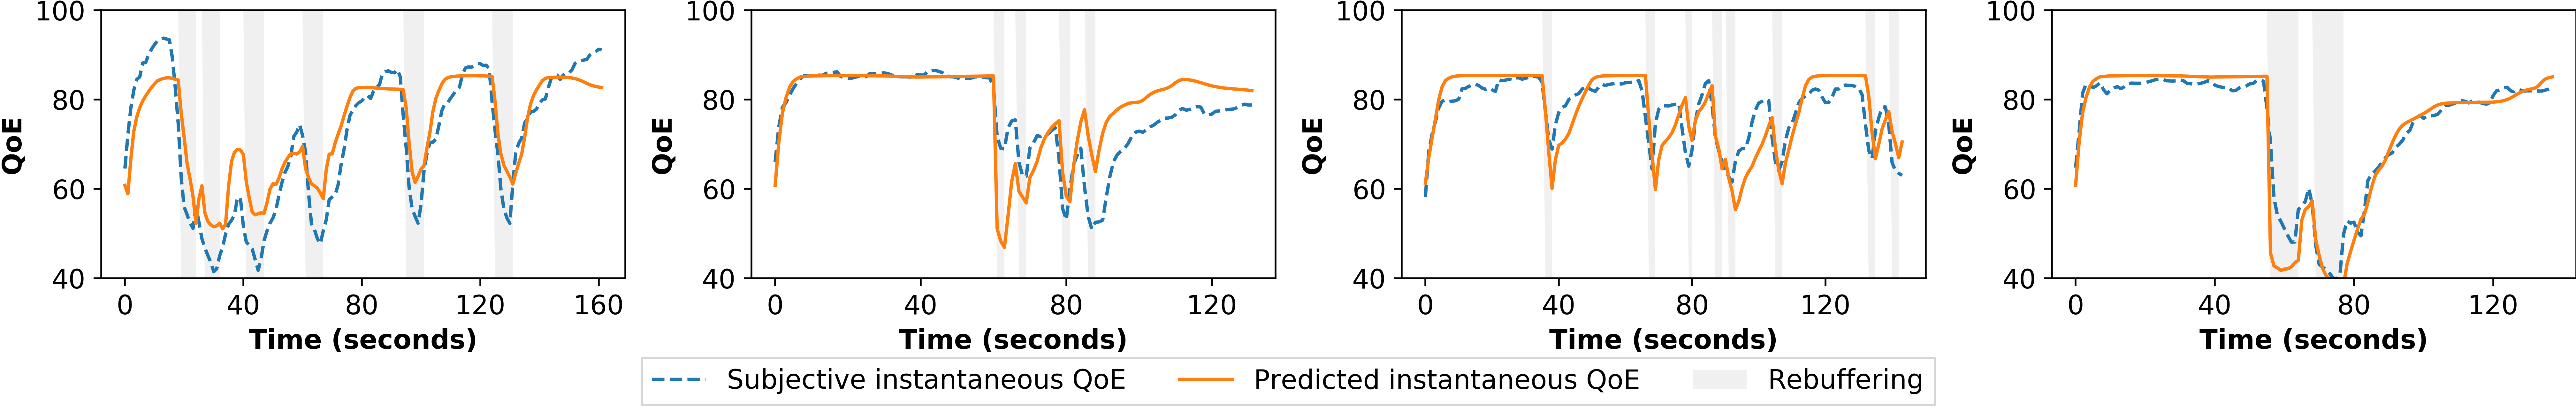
\includegraphics[width=\linewidth]{\FigsDir/lstm_accuracy.png}
  \caption{Some examples of instantaneous QoE prediction performance obtained from the LSTM-QoE model on different test videos of the database.}
  \label{fig:LSTM_Performance}
\end{figure}